\scanpage{40}
% archive foliation: 39
Soit $C$ une catégorie \inserted{$k$-}additive (i.e. additive, munie
de \inserted{homomorphisme} $k\longrightarrow\operatorname{End}(\operatorname{id}_C)$), $C^\bullet$ un complexe \inserted{de cochaînes} dans
$C$
\diagram{\begin{tikzcd}[column sep=small]
0\arrow[r]&C^0\arrow[r,"d^0"]&C^1\arrow[r,"d^1"]&\cdots\arrow[r]&C^i\arrow[r,"d^i"]&C^{i+1}\arrow[r]&\cdots
\end{tikzcd}}
On suppose :
\[
a)\quad\operatorname{Hom}(C^i,C^j)\simeq
\begin{cases}
0&\text{si }j\ne i,i+1,\\
k&\text{si }j=i,\ \text{base }\operatorname{id}_{C^i},\\
k&\text{si }j=i+1,\ \text{base }d^i.
\end{cases}
\]
$b)$ Tout objet de $C$ est isomorphe à une
somme \inserted{finie} d'obj. de la forme $C^i$.

\margin{\figure{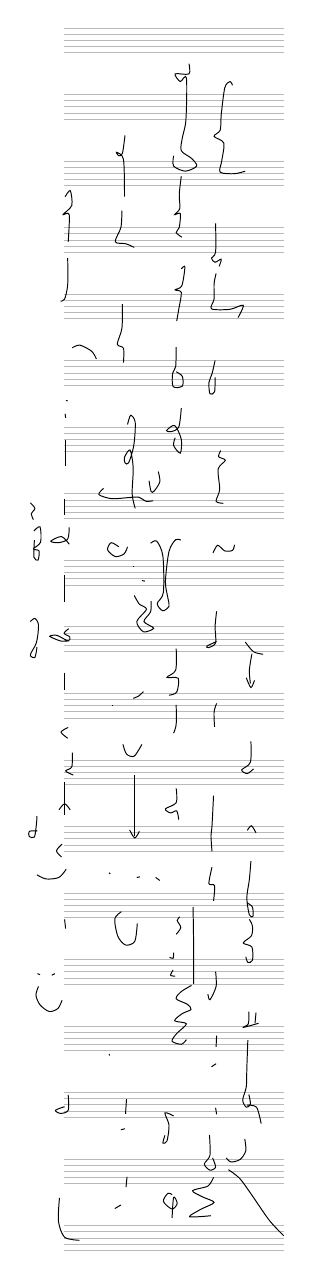
\begin{tikzpicture}[x=.0065cm,y=-.0065cm,line width=.35pt]
\foreach \a in {0,130,260,390,520,650,780,910,1040,1170,1300,1430,1560,1690,1820,1950,2080,2210,2340}{\foreach \b in {0,12,24,36,48}{\draw[gray!55,line width=.12pt] (80,{\a+\b})--(510,{\a+\b});}}
\draw plot[smooth] coordinates {(325,70) (325,90) (298,90) (308,105) (320,98) (319,180) (312,215) (310,240) (330,255) (340,270) (318,280) (295,270) (295,250)};
\draw plot[smooth] coordinates {(410,112) (405,105) (395,117) (388,170) (386,200) (374,212) (393,225) (389,260) (386,282) (414,285) (435,280)};
\draw plot[smooth] coordinates {(200,210) (195,245) (188,250) (183,243) (197,257) (199,330)};
\draw plot[smooth] coordinates {(310,290) (306,325) (307,353) (297,365) (308,363) (306,390) (300,400) (311,409)};
\draw plot[smooth] coordinates {(83,330) (93,318) (96,347) (79,365) (91,365) (89,418)};
\draw plot[smooth] coordinates {(194,357) (192,390) (181,418) (202,422) (218,429)};
\draw plot[smooth] coordinates {(377,382) (377,438) (369,450) (376,458) (388,452) (384,466)};
\draw plot[smooth] coordinates {(88,450) (88,502) (82,530) (74,534)};
\draw plot[smooth] coordinates {(310,471) (317,467) (311,504) (298,512) (310,517) (305,550) (301,573)};
\draw plot[smooth] coordinates {(378,480) (374,500) (374,530) (369,549) (405,550) (431,542) (421,566)};
\draw plot[smooth] coordinates {(195,540) (194,587) (185,618) (197,626) (197,654)};
\draw plot[smooth] coordinates {(97,625) (112,620) (135,632) (144,647)};
\draw plot[smooth] coordinates {(300,624) (299,662) (293,675) (294,701) (312,700) (312,681) (300,672)};
\draw plot[smooth] coordinates {(376,650) (370,676) (364,693) (366,715) (375,711) (376,683)};
\draw plot[smooth] coordinates {(85,728) (88,729)};
\draw plot[smooth] coordinates {(83,754) (84,762)};
\draw plot[smooth] coordinates {(205,775) (211,757) (220,771) (217,817) (207,850) (200,850) (199,839) (210,825) (216,860) (214,911) (220,939)};
\draw plot[smooth] coordinates {(310,743) (305,780) (290,789) (281,787) (297,777) (310,804) (308,831) (295,816) (298,801)};
\draw plot[smooth] coordinates {(84,806) (84,857)};
\draw plot[smooth] coordinates {(387,826) (383,838) (396,845) (382,862) (385,902) (378,925) (392,929)};
\draw plot[smooth] coordinates {(265,867) (268,887) (257,905) (251,906) (247,885)};
\draw plot[smooth] coordinates {(158,900) (149,912) (174,920) (205,918) (227,917) (241,925) (255,924)};
\draw plot[smooth] coordinates {(82,920) (82,952)};
\draw plot[smooth] coordinates {(15,928) (24,939) (17,949) (21,961)};
\draw plot[smooth] coordinates {(22,983) (34,975) (35,1005) (21,1018) (32,1022) (30,1040) (22,1034) (23,1001)};
\draw plot[smooth] coordinates {(91,976) (88,999) (70,1006) (55,1003) (76,994) (91,1009)};
\draw plot[smooth] coordinates {(188,1014) (173,1006) (166,1020) (181,1033) (198,1028) (205,1014)};
\draw plot[smooth] coordinates {(250,1007) (262,1003) (274,1032) (275,1103) (263,1125) (274,1139) (286,1130) (284,1115) (279,1082) (286,1023) (299,1000) (309,1001)};
\draw plot[smooth] coordinates {(372,1026) (381,1011) (395,1022) (410,1021) (414,1010)};
\draw plot[smooth] coordinates {(217,1051) (217,1054)};
\draw plot[smooth] coordinates {(233,1080) (239,1081)};
\draw plot[smooth] coordinates {(81,1070) (81,1121)};
\draw plot[smooth] coordinates {(218,1109) (228,1126) (242,1136) (223,1160) (236,1180) (256,1173) (237,1160) (250,1141) (251,1120)};
\draw plot[smooth] coordinates {(379,1140) (376,1170) (377,1202) (363,1211) (360,1208) (379,1199)};
\draw plot[smooth] coordinates {(15,1160) (24,1154) (31,1167) (27,1201) (15,1225) (24,1230) (28,1210)};
\draw plot[smooth] coordinates {(90,1174) (81,1183) (92,1190) (89,1198) (67,1187) (53,1189) (74,1198) (88,1198)};
\draw plot[smooth] coordinates {(435,1200) (451,1219) (470,1224)};
\draw plot[smooth] coordinates {(448,1223) (443,1255) (445,1281)};
\draw plot[smooth] coordinates {(437,1270) (446,1289) (453,1275)};
\draw plot[smooth] coordinates {(300,1213) (299,1255) (282,1269) (304,1271) (301,1298) (286,1304)};
\draw plot[smooth] coordinates {(82,1260) (82,1294)};
\draw plot[smooth] coordinates {(236,1297) (226,1306) (216,1310)};
\draw plot[smooth] coordinates {(174,1324) (177,1324)};
\draw plot[smooth] coordinates {(300,1323) (300,1361) (295,1378)};
\draw plot[smooth] coordinates {(379,1320) (374,1337) (375,1366)};
\draw plot[smooth] coordinates {(89,1367) (75,1376) (88,1388)};
\draw plot[smooth] coordinates {(196,1400) (203,1419) (218,1423) (233,1400)};
\draw plot[smooth] coordinates {(97,1416) (96,1444) (84,1452) (99,1460)};
\draw plot[smooth] coordinates {(446,1394) (445,1435) (428,1450) (439,1457) (451,1448)};
\draw plot[smooth] coordinates {(218,1460) (218,1510) (218,1580)};
\draw plot[smooth] coordinates {(209,1567) (219,1583) (228,1570)};
\draw plot[smooth] coordinates {(300,1486) (300,1514) (279,1526) (289,1534) (301,1530) (305,1547)};
\draw plot[smooth] coordinates {(82,1474) (82,1538)};
\draw plot[smooth] coordinates {(71,1528) (82,1516) (93,1528)};
\draw plot[smooth] coordinates {(28,1540) (27,1555) (23,1581) (13,1580) (13,1570) (29,1569)};
\draw plot[smooth] coordinates {(77,1595) (66,1608) (76,1620)};
\draw plot[smooth] coordinates {(85,1644) (71,1660) (46,1663) (28,1655)};
\draw plot[smooth] coordinates {(373,1500) (370,1559) (368,1579) (370,1609)};
\draw plot[smooth] coordinates {(439,1568) (447,1559) (456,1573)};
\draw plot[smooth] coordinates {(370,1640) (364,1672) (375,1676) (373,1706)};
\draw plot[smooth] coordinates {(446,1628) (443,1664) (438,1700) (443,1733) (450,1736) (449,1718) (439,1710)};
\draw plot[smooth] coordinates {(169,1651) (171,1653)};
\draw plot[smooth] coordinates {(223,1660) (229,1659)};
\draw plot[smooth] coordinates {(260,1660) (268,1666)};
\draw plot[smooth] coordinates {(193,1727) (180,1741) (186,1775) (201,1792) (219,1785) (224,1750)};
\draw plot[smooth] coordinates {(82,1742) (84,1760)};
\draw plot[smooth] coordinates {(307,1737) (302,1744) (309,1758) (300,1771)};
\draw plot[smooth] coordinates {(333,1718) (334,1789) (334,1868)};
\draw plot[smooth] coordinates {(443,1742) (449,1755) (447,1774) (431,1788) (448,1796) (449,1822) (440,1826) (436,1815)};
\draw plot[smooth] coordinates {(295,1807) (294,1818) (287,1816)};
\draw plot[smooth] coordinates {(294,1841) (289,1851) (298,1853)};
\draw plot[smooth] coordinates {(29,1848) (34,1850)};
\draw plot[smooth] coordinates {(57,1851) (63,1848)};
\draw plot[smooth] coordinates {(31,1873) (26,1890) (34,1909) (52,1922) (69,1916) (77,1900)};
\draw plot[smooth] coordinates {(330,1871) (310,1883) (300,1897) (322,1908) (329,1918) (312,1926) (297,1940) (320,1946) (301,1965) (292,1980) (310,1986) (320,1977)};
\draw plot[smooth] coordinates {(377,1844) (378,1873) (366,1899) (362,1888)};
\draw plot[smooth] coordinates {(442,1922) (441,1946) (431,1953) (461,1945)};
\draw plot[smooth] coordinates {(456,1924) (454,1945)};
\draw plot[smooth] coordinates {(379,1969) (378,1991)};
\draw plot[smooth] coordinates {(378,2024) (369,2030)};
\draw plot[smooth] coordinates {(169,2005) (170,2008)};
\draw plot[smooth] coordinates {(440,1978) (438,2034) (437,2069) (430,2095) (437,2109) (445,2103) (442,2084)};
\draw plot[smooth] coordinates {(89,2085) (89,2115) (74,2121) (64,2115) (82,2108)};
\draw plot[smooth] coordinates {(203,2093) (201,2122)};
\draw plot[smooth] coordinates {(200,2151) (192,2153)};
\draw plot[smooth] coordinates {(295,2126) (278,2120) (286,2144) (282,2175) (274,2179) (278,2164)};
\draw plot[smooth] coordinates {(377,2110) (379,2123)};
\draw plot[smooth] coordinates {(365,2163) (366,2203) (355,2220) (366,2232) (377,2226) (371,2208)};
\draw plot[smooth] coordinates {(434,2171) (436,2194) (425,2211) (407,2216) (398,2208)};
\draw plot[smooth] coordinates {(438,2105) (457,2109) (466,2141)};
\draw plot[smooth] coordinates {(204,2245) (202,2265)};
\draw plot[smooth] coordinates {(192,2300) (180,2307)};
\draw plot[smooth] coordinates {(292,2280) (284,2277) (275,2293) (292,2308) (302,2297) (295,2285) (292,2325)};
\draw plot[smooth] coordinates {(373,2246) (362,2263) (332,2272) (351,2284) (374,2295) (349,2308) (326,2323) (368,2321)};
\draw plot[smooth] coordinates {(72,2286) (70,2332) (82,2363) (111,2369)};
\draw plot[smooth] coordinates {(402,2231) (424,2248) (446,2278) (482,2330) (510,2360)};
\end{tikzpicture}}}
% crop-candidate: scan 40

Soit $A$ la sous-catégorie pleine de $C$
formée des \deleted{\unsure{\Phi}} $C^i$; elle n'est pas additive,
mais tout de même \unsure{structure|strictement} $k$-linéaire,
i.e. les $\operatorname{Hom}_A$ sont des $k$-modules, leurs
compositions est $k$-bil.

\deleted{\unsure{L}}L'existence de $(C,C^\bullet)$ satisfaisant $a)$
$b)$ est immédiate par construction ``abstraite''.
On peut aussi réaliser $C$ comme la cat. (des
complexes de chaînes \inserted{$L_*$} de $k$-modules
satisfaisant les conditions

$1^\circ)$ \deleted{\unsure{le}} $L_*$ est acyclique i.e. $H_i(L_*)=0$ $\forall i\geqslant0$.

$2^\circ)$ $L_n$ et $Z_n(L_*)$ sont libres de t.f. pour $\forall n$.

$3^\circ)$ $L_n$ est nul pour $n$ grand.

On prendra alors :
\[
C^i=\deleted{\unsure{K(C^i_*)}}C^i_*=\left\{
\begin{gathered}
\cdots\ 0\ \cdots\
\overset{\text{deg }i+1}{k}\xrightarrow{\mathrm{id}}
\overset{\text{deg }i}{k}\longrightarrow0\ \cdots\longrightarrow
\overset{\text{deg }0}{0}
\end{gathered}\right\}
\]
i.e. les comp. sont nulles sauf en degrés $i,i+1$ où
on a $k$, et l'op. diff. \unsure{$d_{i+1}$} est l'identité.
On prend $C^i_*\xrightarrow{d^i}C^{i+1}_*$ caractérisé
par $(d^i)_{i+1}=\operatorname{id}_k$. Les conditions $a)$ et $b)$ sont
satisfaites trivialement. On pourrait aussi
\unsure{prendre} des complexes de cochaînes : le plus,
